% !TEX root =  ../main.tex

\chapter{Introduction} \label{ch:introduction}

	General Aviation (GA) is one of two branches of Civil Aviation, which pertains to the operation of all non-scheduled and non-military aircraft~\cite{aopa2009what,allen2006general,federal-aviation-administration2016the-economic,kenny201726th}.  GA includes fixed-wing airplanes, helicopters (rotorcraft), balloons, dirigibles, gliders, etc.; and comprises 63\% of all Civil Aviation activity within the U.S.~\cite{aopa2009what,federal-aviation-administration2016the-economic,shetty2012current}.  Performing GA flight analysis is essential for making the GA community safer, as currently GA has the highest accident rates in Civil Aviation~\cite{kenny201726th,aopa-air-safety-institute20172015-2016}.  As of 2014, the total accident and fatality rates for GA fixed-wing aircraft were 5.78 and 1.19 per 100,000 flight hours, respectively; and 75.3\% of GA accidents were caused by pilot-related actions~\cite{kenny201726th}.

	The National General Aviation Flight Information Database (NGAFID) has been developed at the University of North Dakota as a joint university-industry-FAA initiative that is responsible for the curation, dissemination, and analysis of flight data for the General Aviation (GA) sector of Civil Aviation~\cite{clacharlarge-scale,url_ngafid}.  The objective of the NGAFID is to proactively identify accident precursors and mitigate risks associated with unsafe flight practices and aircraft maintenance issues within the GA community.  This is achieved via non-punitive information sharing to educate operators on risks associated with their flights to encourage safer practices~\cite{clacharlarge-scale}.  The analytical tools provided by the NGAFID are free and available to GA pilots who participate by uploading their flight data through the NGAFID web application\footnote{http://www.ngafid.com} or the GAARD mobile application~\cite{url_gaard}.  Subsequently, their flight data is preprocessed and analyzed using various queries.  Many queries are based on threshold criteria called \textit{exceedances}, which are predefined using known limitations of the make/model aircraft or the phase of flight. However, other recent work has focused on developing more advanced analytics through machine learning and other holistic techniques~\cite{sophine2014identifying,sophine2016phd,desell2015evolving,elsaid2016vibration,elsaid2016thesis,desell2014evolving,elsaid2018using}.  Upon logging into the web portal, the user is provided with summaries of any unsafe events (see \Cref{fig:exceedance_example}) and is able to reanimate their flight(s) using X-Plane\footnote{http://www.x-plane.com} or Cesium\footnote{http://www.cesiumjs.org} (see \Cref{fig:cesium_example}).  The intent is to educate participating pilots on any unsafe practices in their flight and maintenance issues with the aircraft which may contribute to an accident/incident. The overall goal of this initiative is to reduce the accident and fatality rates within the GA community.

	\begin{figure}
    	\centering
        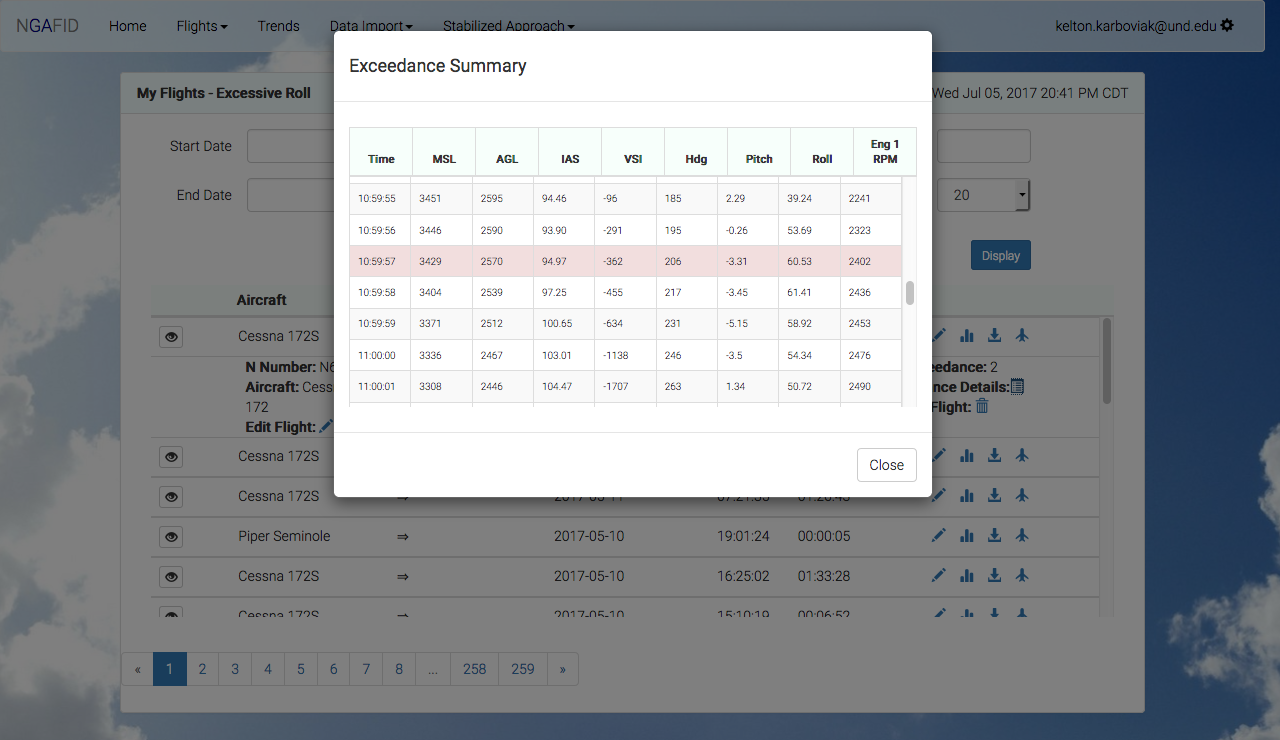
\includegraphics[width=\linewidth]{exceedance_example.png}
        \caption{Screen-shot of a flight which has an excessive roll exceedance.  The exceedance event is highlighted in red.}
        \label{fig:exceedance_example}
    \end{figure}
    
    \begin{figure}
    	\centering
        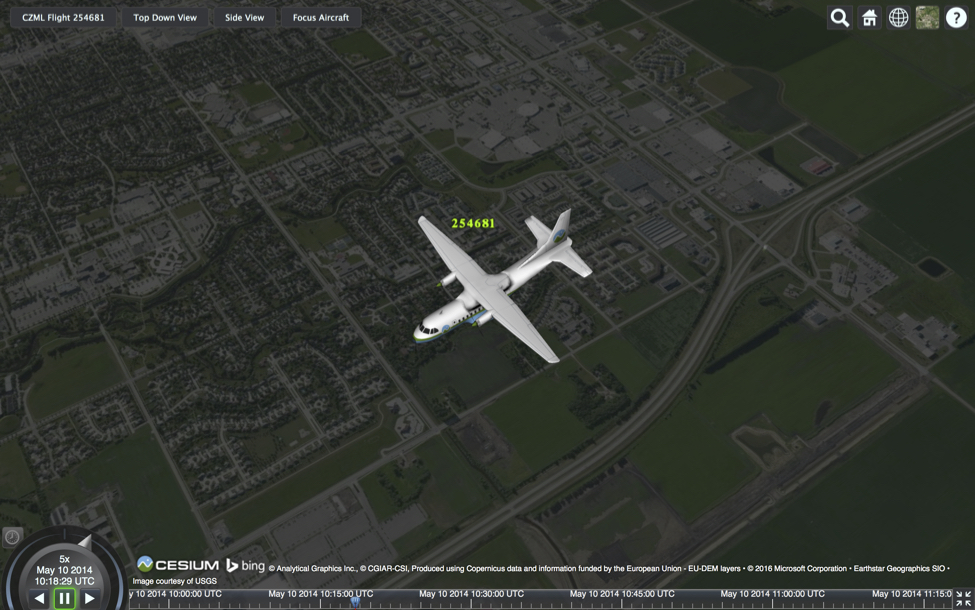
\includegraphics[width=\linewidth]{cesium_example.jpg}
        \caption{Example of in-browser flight reanimation using Cesium.}
        \label{fig:cesium_example}
    \end{figure}


%----------------------------------------
% SCOPE & OBJECTIVES
%----------------------------------------
\section{Scope \& Objectives} \label{sec:objectives}

	The goal of this research is to develop an automated grading system, the \toolname\ (\toolnameshort), for analyzing quality of approach and landing phases with a low error rate, reasonable run-time, and that can handle the wide variation of GA flight.  This application will be useful in several different areas:
%
    \begin{itemize}
    	\item provide student pilots with a grade/metric that they can use to gauge a flight's quality, which helps target different student learning techniques,
        \item help improve the flight training process for Certified Flight Instructors (CFI) by making post-flight evaluation more efficient,
        \item help reduce costs of training for the student and institution due to a lesser need for additional training flights, and
        \item help further reduce GA accident and fatality rates.
    \end{itemize}
    

%----------------------------------------
% MOTIVATION
%----------------------------------------
\section{Motivation} \label{sec:motivation}

	Despite many safety efforts that have been recently introduced to the GA community, accident rates in the United States remain high.  One way of characterizing flight safety is by identifying \textit{exceedances}, or events that bring the aircraft into an unsafe state dependent on the phase of flight.  By detecting these exceedances, we can identify areas of improvement at the pilot- or organizational-level and additionally educate the pilots on their unsafe practices.  In particular, this research is mainly focused on this aspect of improving teaching feedback for Certified Flight Instructors (CFIs) and student pilots within flight training institutions (although it may be useful to individual private pilots as a side-effect).  Furthermore, the scope of analysis is for the approach and landing phases of flight since these are some of the most critical phases in GA as they ranked \#6 and \#1, respectively, for number of pilot-related accident types in 2014~\cite{kenny201726th}.  These phases present particular challenges in detection of the phase and exceedances due to the high variability in GA operations and flight performance~\cite{goblet2015identifying,goblet2016phase,fala2016detecting}.
    
    At the time of this writing, the feedback that a student pilot receives for their flying performance consists of a verbal debriefing given by the student's CFI.  This process can be prone to errors as both the CFI and student must recall the flight from memory or utilize any notes they were able to take mid-flight.  Additionally, a cross-country flight may last anywhere from 1.5 to 2 hours, which can be a lot to recall after they have landed and returned the aircraft.  This may work well for some students, but not for all as many people do not have a great short-term memory.  For these reasons, an automated system that can provide metrics-based results of their flying performance and allow them to replay their flight will benefit student pilots by providing another means of obtaining feedback, which will cater to students who learn more efficiently with visual materials.


%----------------------------------------
% OUTLINE
%----------------------------------------
\section{Outline} \label{sec:outline}

	This thesis is organized with related works in the areas of aircraft operations, post-flight evaluation tools, NGAFID related work, and data mining techniques in \Cref{ch:related_work}.  \Cref{ch:methodology,ch:implementation} are a continuation of previous work presented in~\cite{karboviak2018classifying}.  The approach to phase of flight identification, exceedance detection, grading, and web interface are discussed in \Cref{ch:methodology}.  The implementation; including the programming languages, libraries, and parallelization techniques used; are discussed in \Cref{ch:implementation}.  Results of the flight analysis are given in \Cref{ch:results}.  Finally, there is a conclusion of the research and a discussion of future work in \Cref{ch:conclusion}.
    
    
    
